\section{Question 4}

\subsection{Question}
\verbatiminput{q4/q4.txt}

\subsection{Answer}

With the code in Listing \ref{listing:scaledownmain}, multidimensional scaling (MDS) was used to create a two-dimensional visualization of the blog distance graph. This code calls the {\tt scaledown} function, which is shown in Listing \ref{listing:scaledownfunc}. The algorithm continues until the error factor stops decreasing, as shown in the output in Appendix A, Listing \ref{scaledown}. 

\lstinputlisting[language=Python, caption={main for scaledown}, label=listing:scaledownmain,linerange={301-302},firstnumber=301]{clusters.py}

\lstinputlisting[language=Python, caption={scaledown function}, label=listing:scaledownfunc,linerange={224-272},firstnumber=224]{clusters.py}

The {\tt scaledown} function returns the coordinates for each of the blogs in 2D space. This data was then used with the {\tt draw2d} function in Listing \ref{listing:draw2d}, which produced the two-dimensional visualation created from the MDS algorithm, as shown in Figure \ref{fig:blogs2d}.

\lstinputlisting[language=Python, caption={draw2d function}, label=listing:draw2d,linerange={274-281},firstnumber=274]{clusters.py}

\begin{figure}[h!]
\centering
\fbox{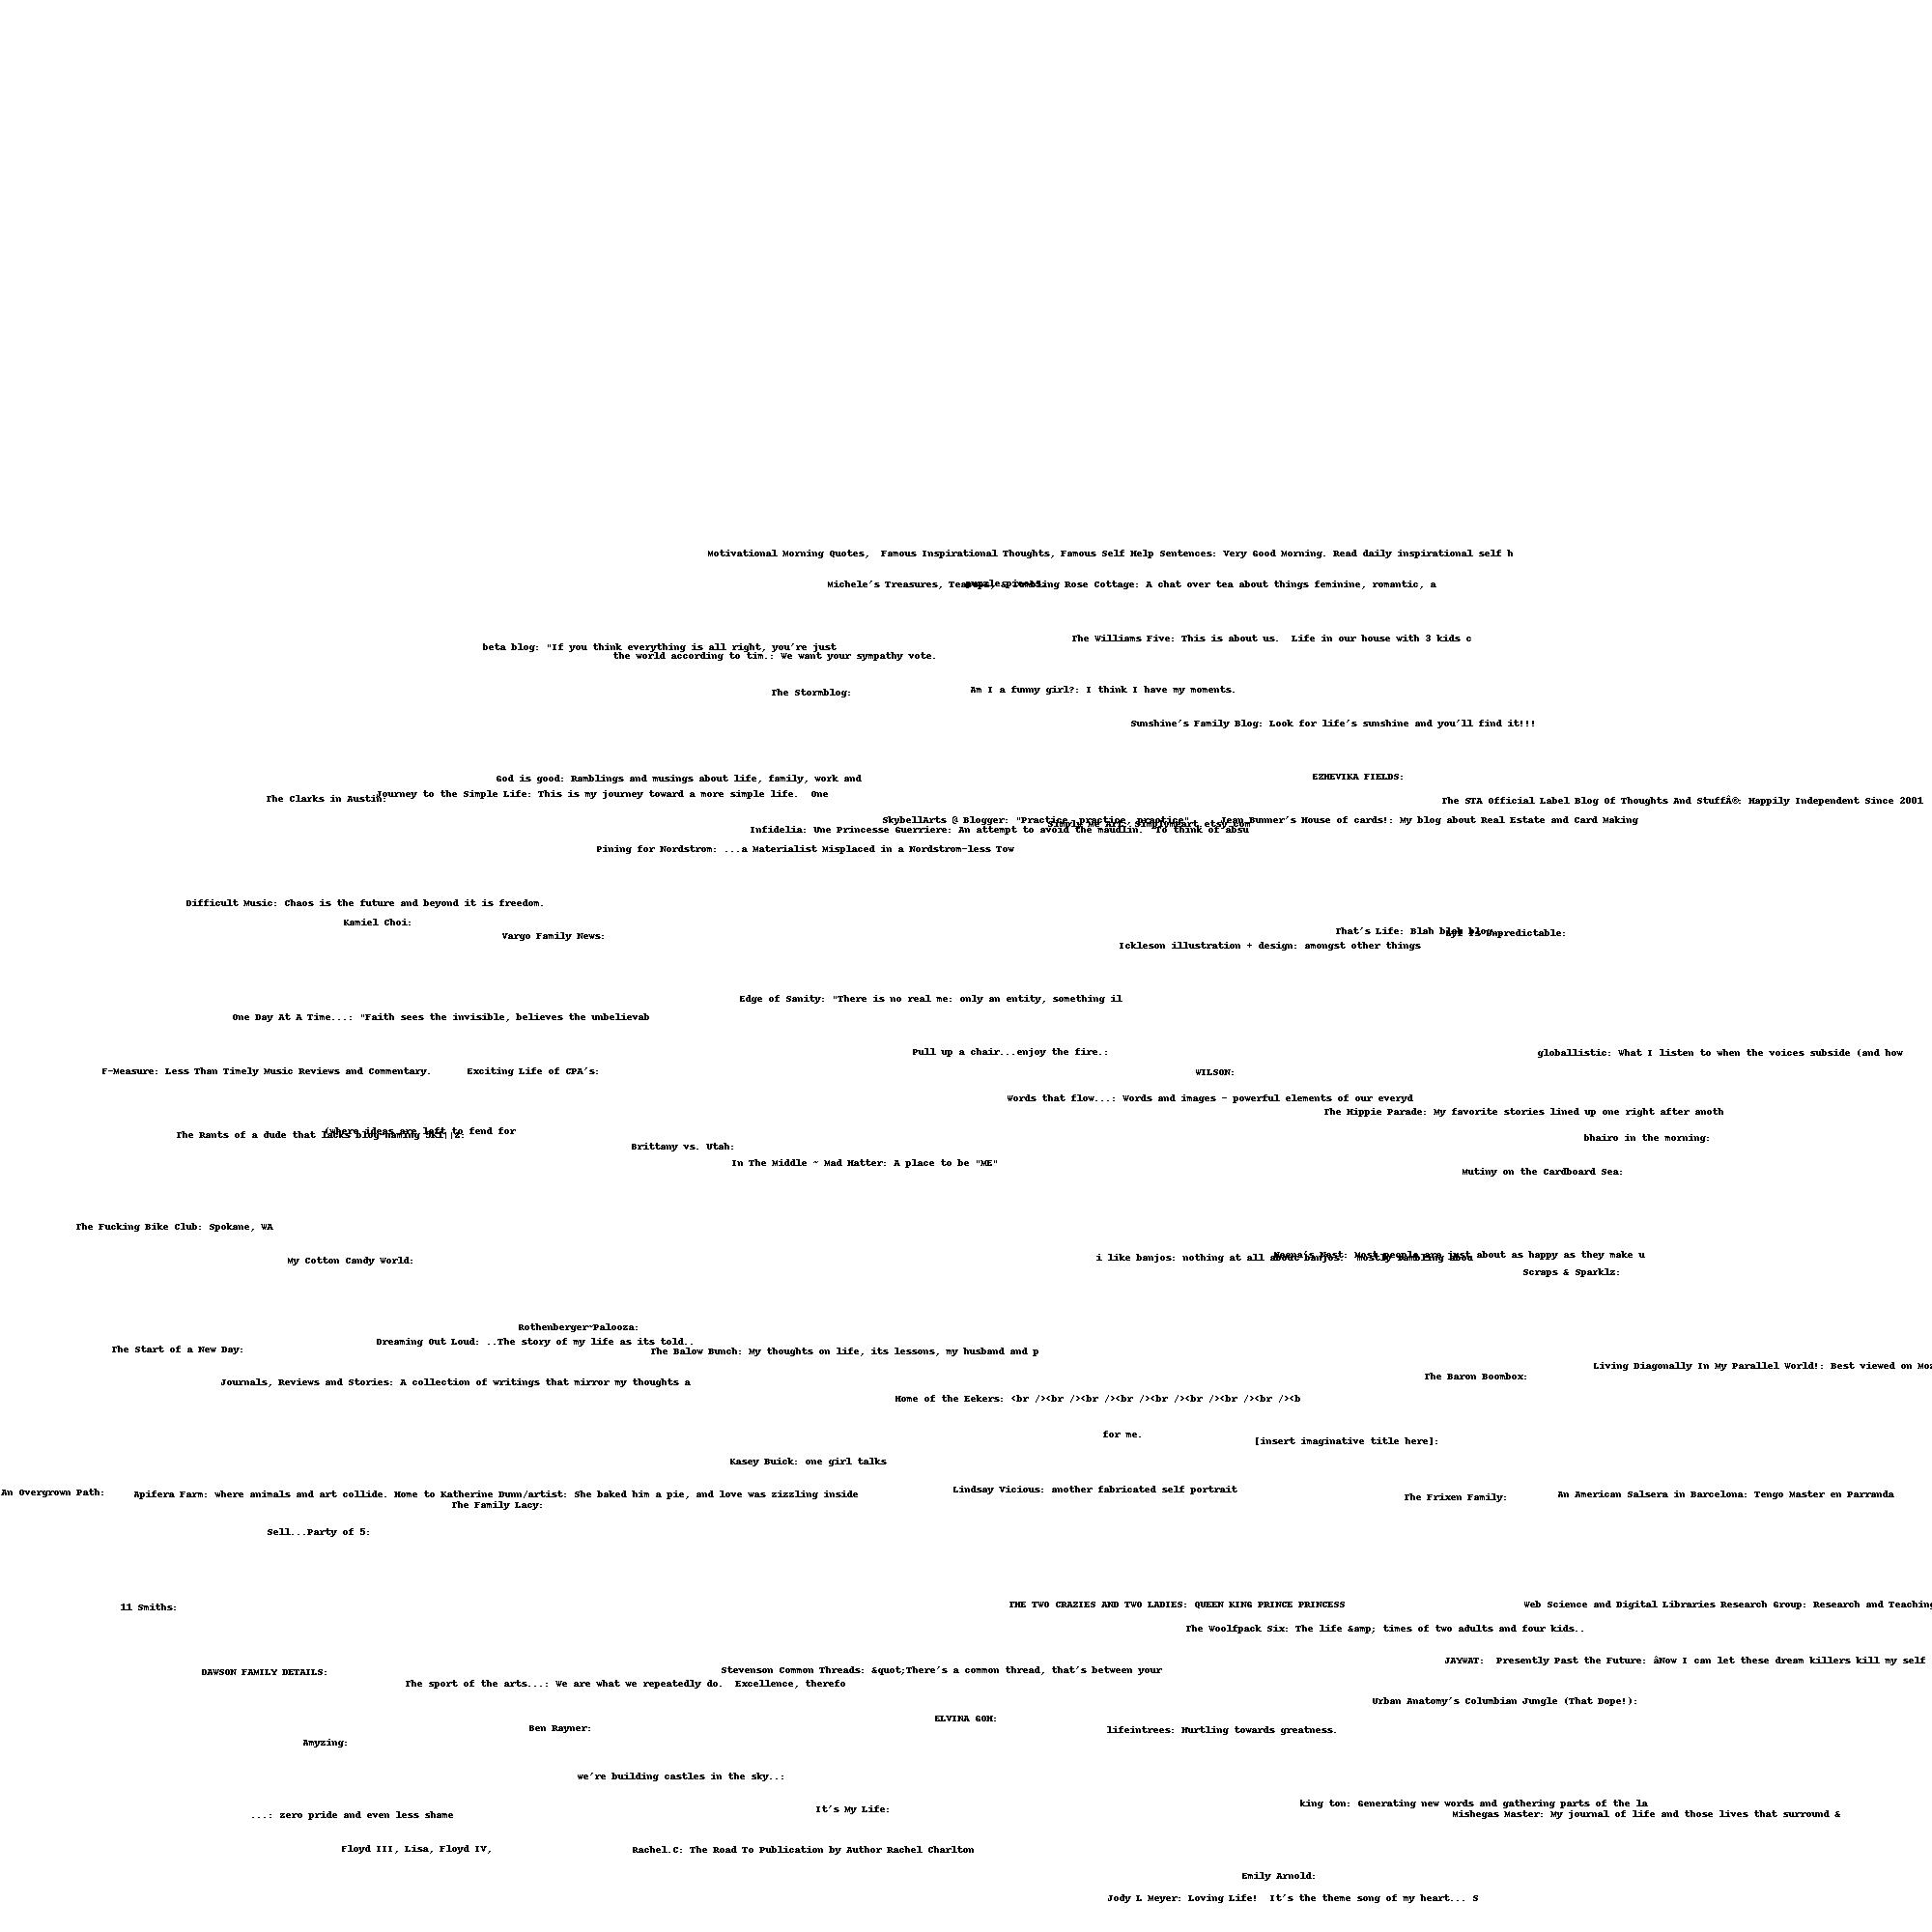
\includegraphics[trim=0 0 0 500, clip, scale=0.2]{q4/blogs2d.jpg}}
\caption{MDS 2d visualization}
\label{fig:blogs2d}
\end{figure}